\documentclass[11pt]{article}
\usepackage{graphicx}
\usepackage{booktabs}
\usepackage{siunitx}
\usepackage{caption}
\usepackage{geometry}
\usepackage{enumitem}
\geometry{margin=1in}

\title{Exploratory Data Analysis Narrative\\PhysioNet 2012 ICU Cohort}
\author{Computational Stats Project}
\date{\today}

\begin{document}
\maketitle

\section{Cohort and Notebook Context}
The notebook \texttt{physionet\_eda.ipynb} loads the PhysioNet/Computing in Cardiology 2012 Challenge training cohort (``set-a''). It contains 4{,}000 ICU stays, each with a general descriptor row and a patient-specific time-series file. Data access is handled through \texttt{dataloader.py} utilities to keep consistency with the rest of the repository. All figures referenced below are saved automatically in \texttt{figures/} when the notebook runs.

\section{Demographic Descriptors}
Figure~\ref{fig:demo} provides three complementary perspectives:
\begin{itemize}[noitemsep]
    \item Age: unimodal distribution centered in the early 60s with long tails toward both younger trauma patients and very old patients. A kernel density overlay highlights mild right skew consistent with ICU populations.
    \item Gender: the notebook remaps the binary indicator to \{Female, Male\} and counts occurrences. The bars show a modest male majority (~55\%).
    \item ICU type: integer-coded categories are mapped to descriptive labels (CCU, Cardiac Surgery Recovery, MICU, SICU). The bar plot confirms representation across cardiac and medical units, implying heterogeneous case mix.
\end{itemize}
The underlying summary statistics (Cell 6 output) include mean, standard deviation, and quartiles for Age, Height, Weight, and ICUType. These tabular descriptors are not reproduced verbatim here but should accompany Figure~\ref{fig:demo} when presenting results.

\begin{figure}[h]
    \centering
    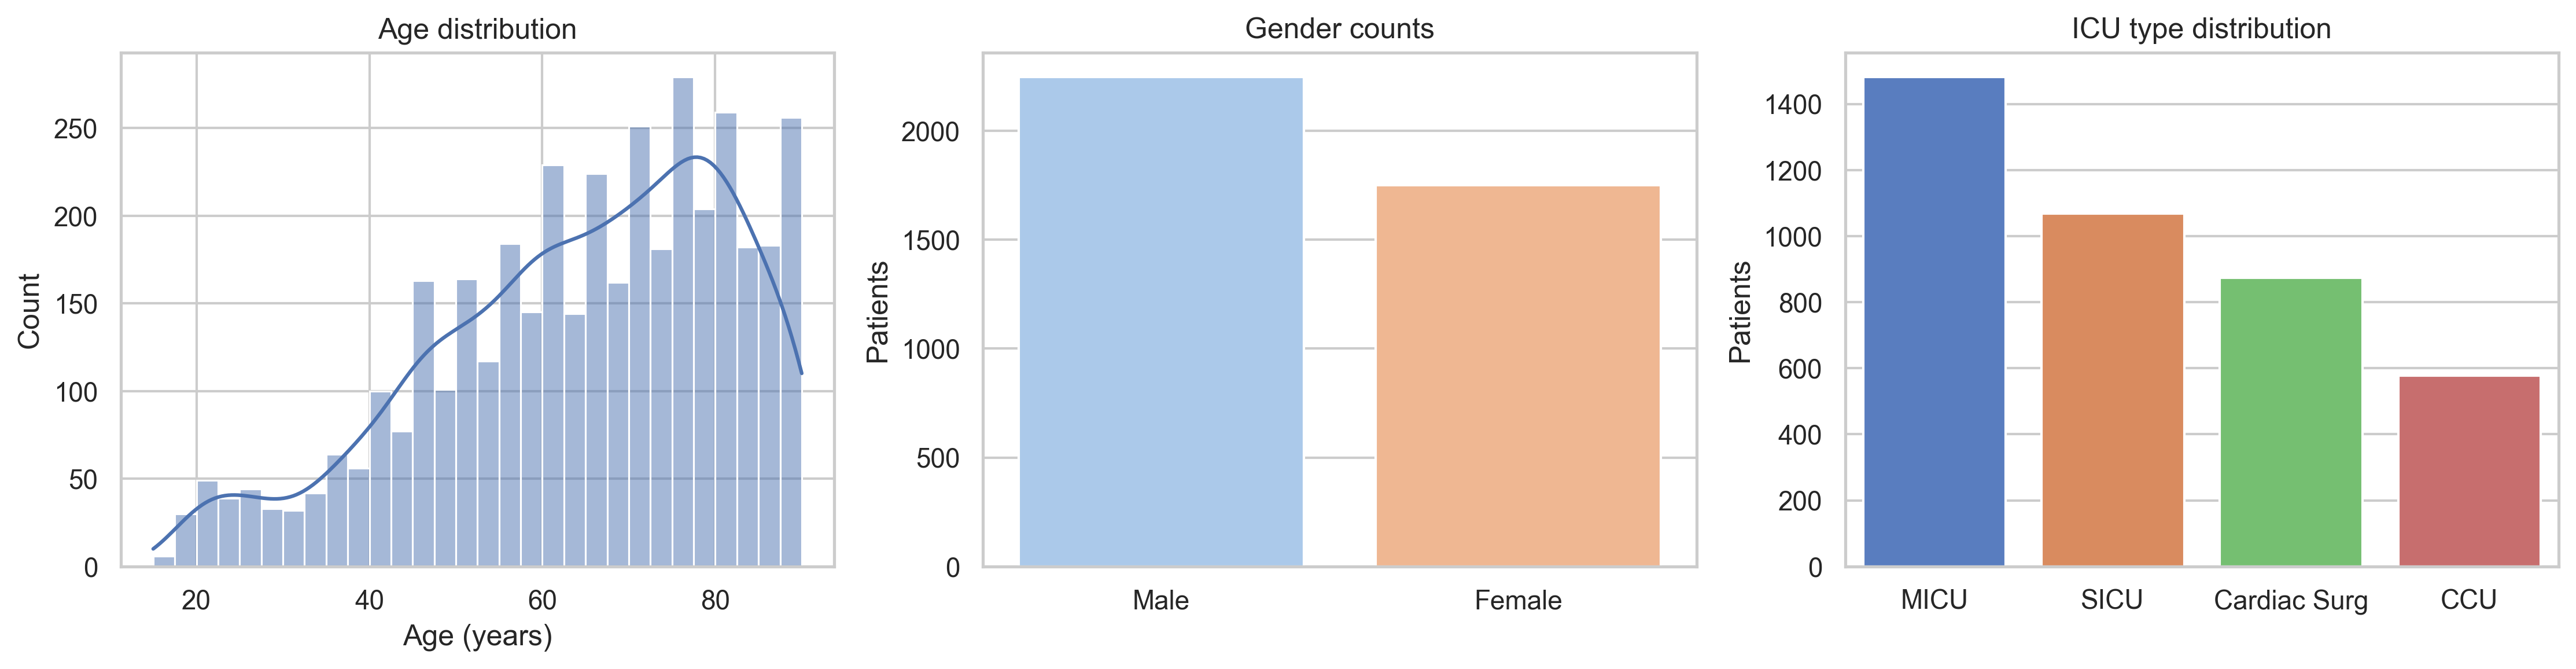
\includegraphics[width=0.85\textwidth]{figures/demographic_distributions.png}
    \caption{Age histogram, gender counts, and ICU-type distribution for the cohort.}
    \label{fig:demo}
\end{figure}

\section{Measurement Density}
Figure~\ref{fig:meas} shows the histogram of charted rows per stay. The inline summary statistics (Cell 9 output) report quartiles; for example, the median patient has roughly 1{,}400 chart rows while the upper quartile exceeds 2{,}500 rows. This variability motivates downstream handling strategies (e.g., resampling, time-bucketing, or masking) discussed in other modules of the repository.

\begin{figure}[h]
    \centering
    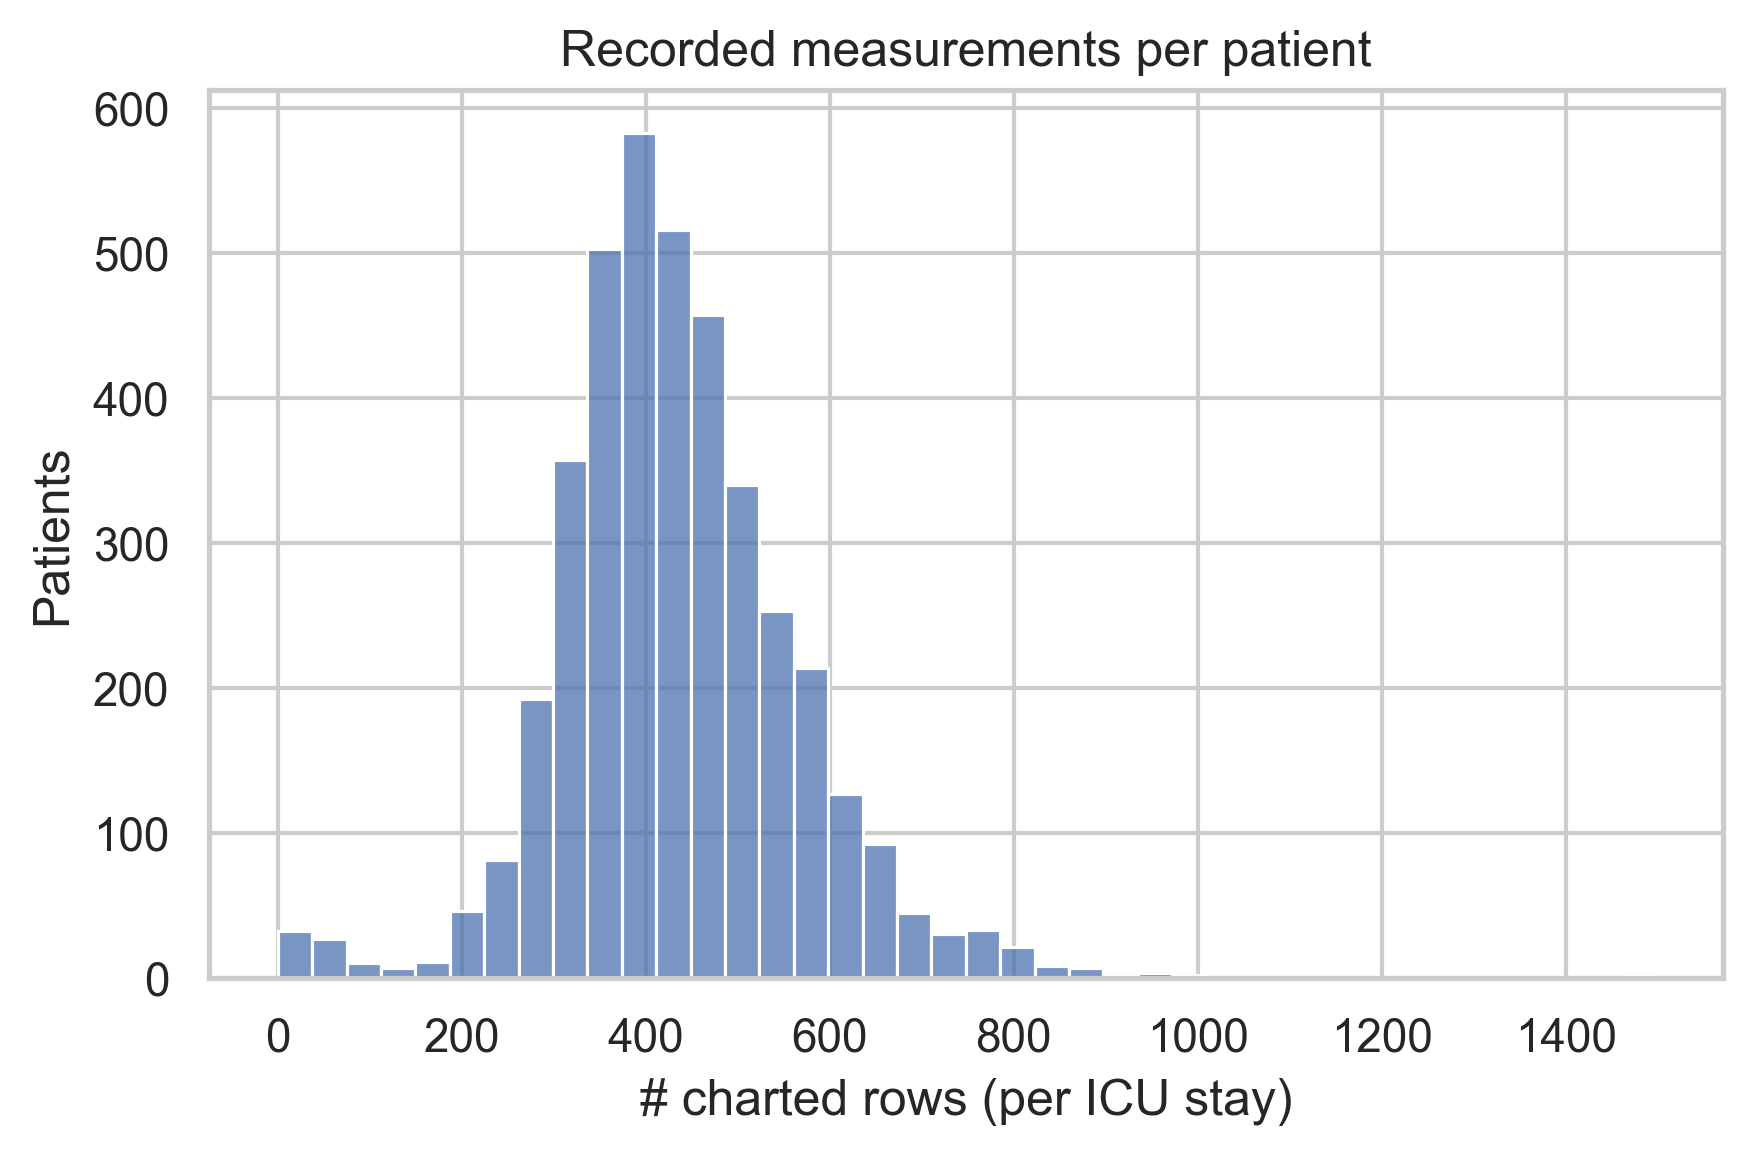
\includegraphics[width=0.65\textwidth]{figures/measurement_count_distribution.png}
    \caption{Distribution of recorded measurement counts per ICU stay.}
    \label{fig:meas}
\end{figure}

\section{Feature Missingness Landscape}
Figure~\ref{fig:missingness} orders all time-series variables from most complete (bottom) to sparsest (top). Vitals such as HR, MAP, and SaO$_2$ approach full coverage, whereas labs (Creatinine, Lactate) have higher missing rates. The plotted data originate from \texttt{compute\_feature\_missingness} and are tabulated in \texttt{missingness\_df}. Presenting this plot alongside the table assists in selecting robust feature subsets or defining imputation rules.

\begin{figure}[h]
    \centering
    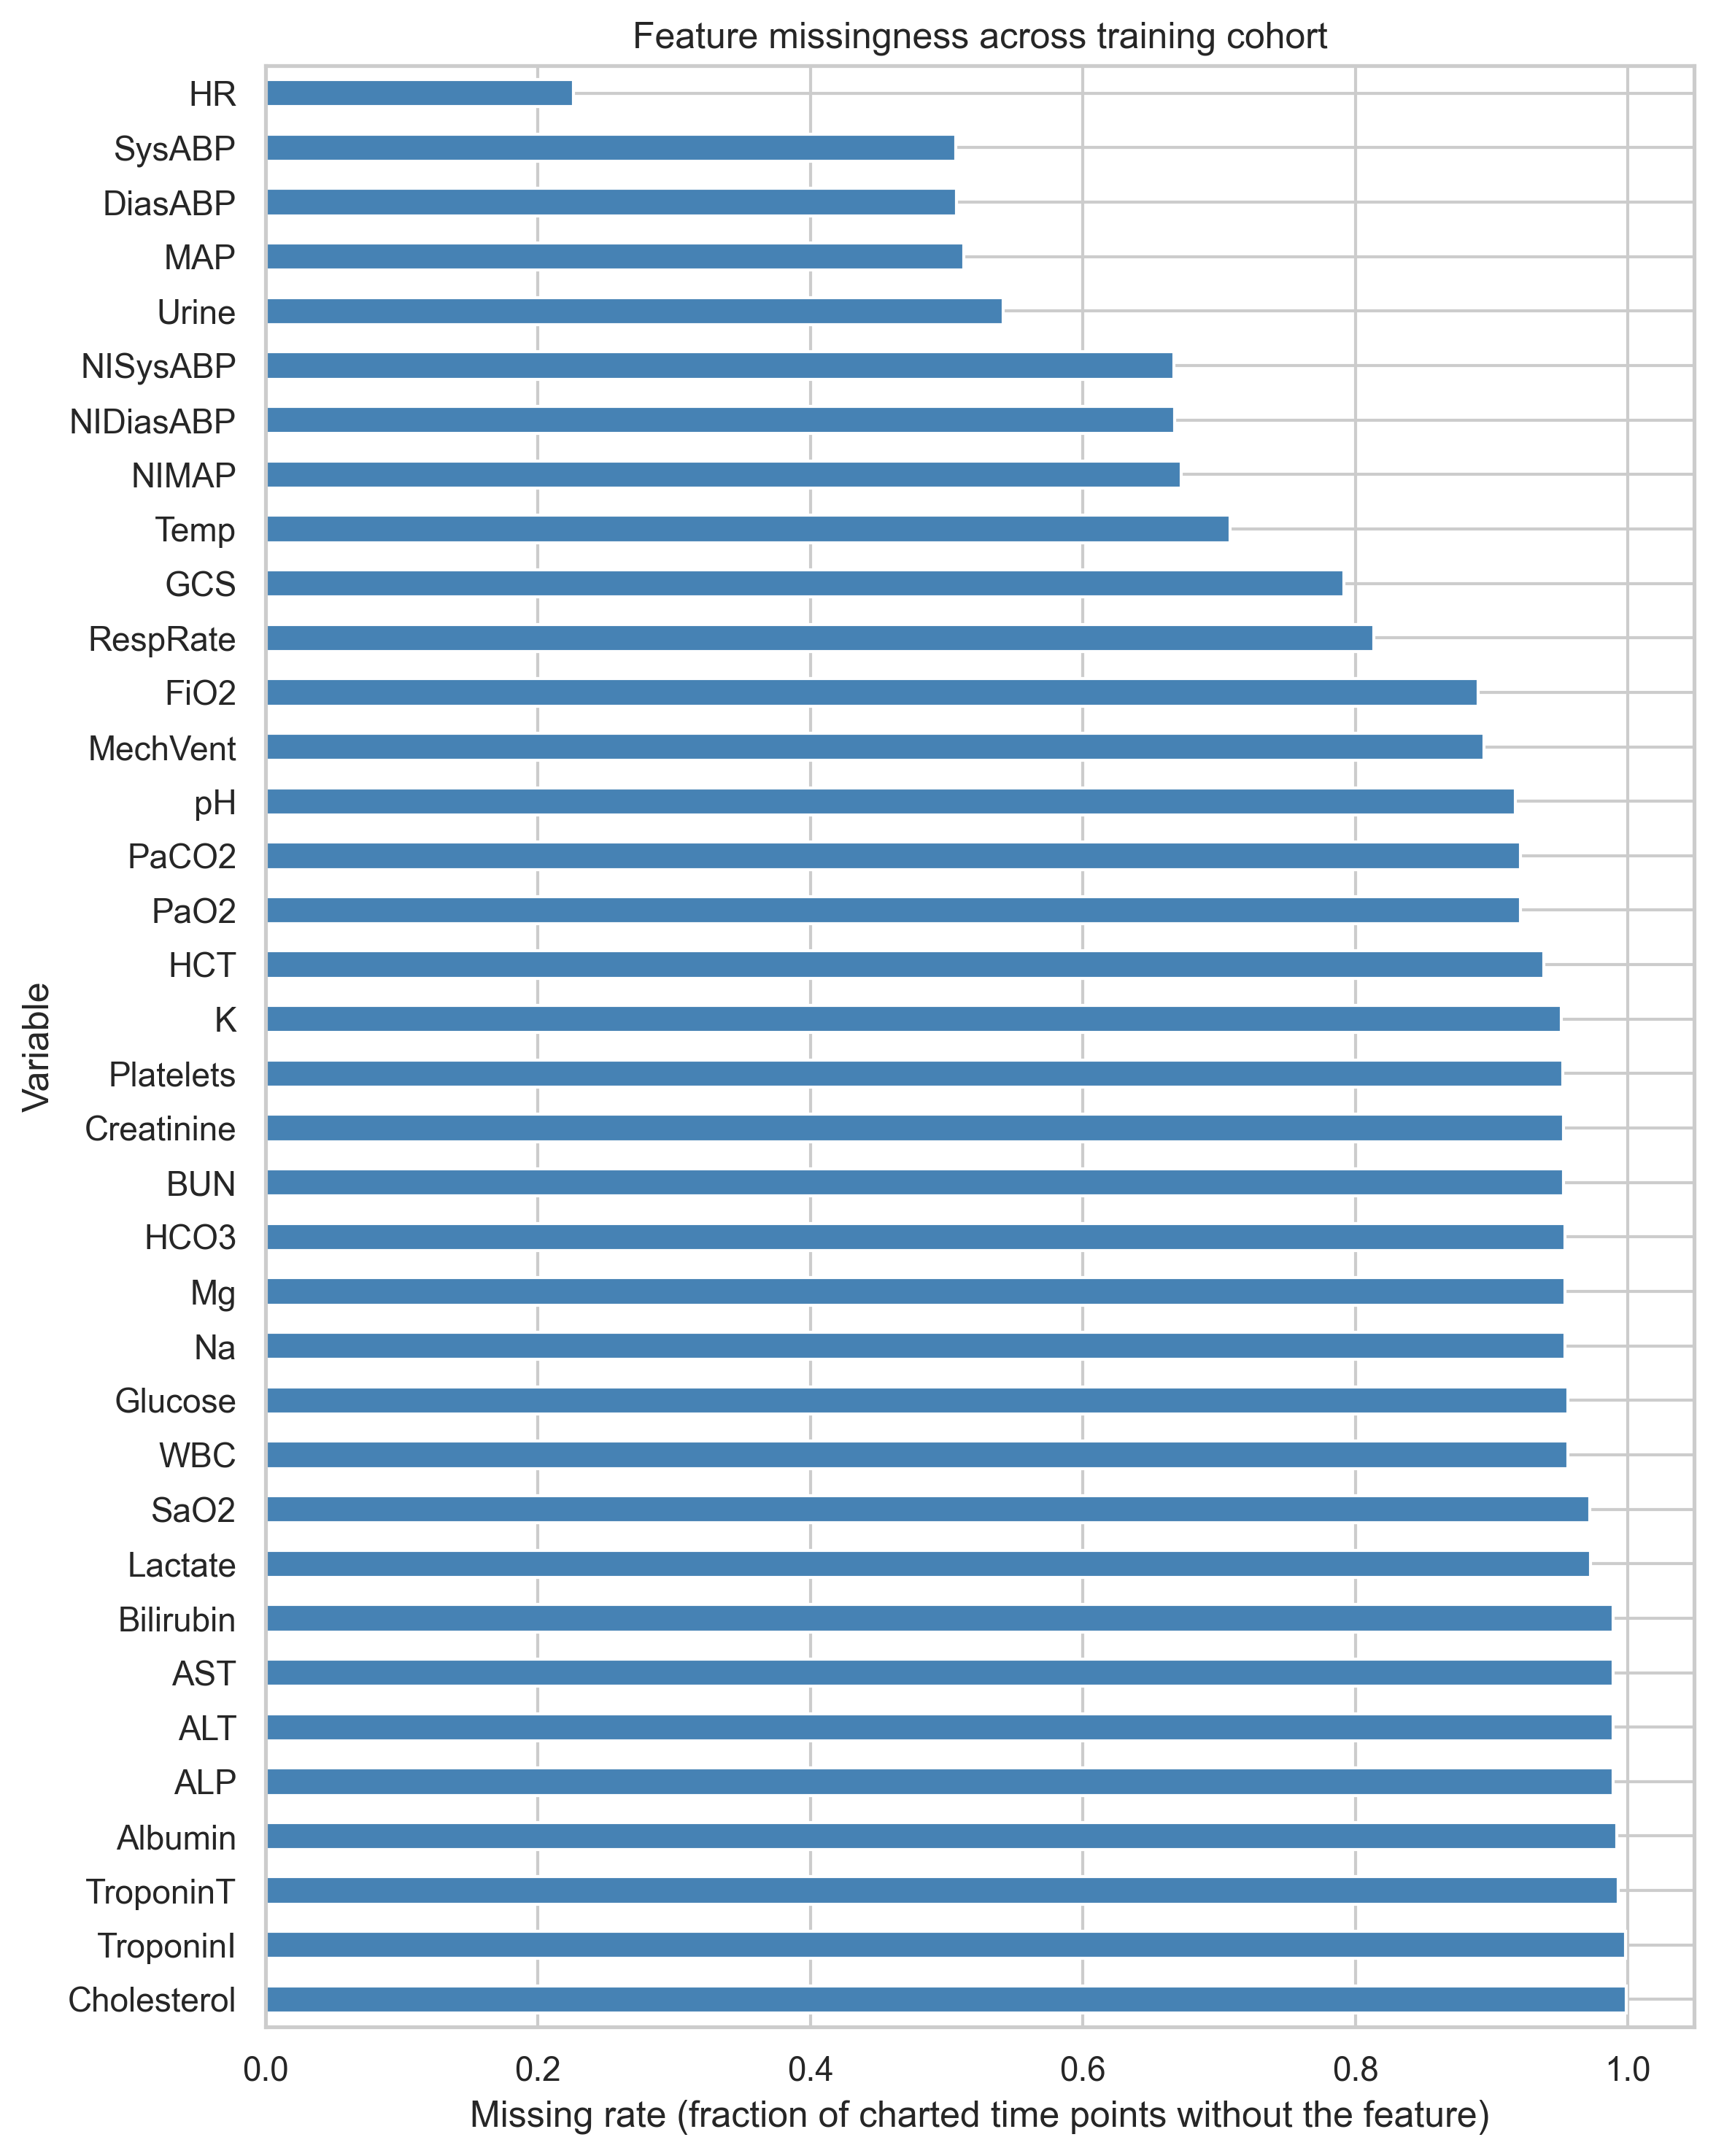
\includegraphics[width=0.75\textwidth]{figures/feature_missingness.png}
    \caption{Missing rate per variable across the 4{,}000 admission time series.}
    \label{fig:missingness}
\end{figure}

\section{Representative Trajectory}
Figure~\ref{fig:trajectory} plots HR, SysABP, DiasABP, and RespRate for the single patient with the densest time series. Subplots share the time axis and use markers to emphasize irregular sampling. The figure is paired with a short table (Cell 14 output) showing the first rows of the pivoted wide table for the selected variables. This vignette provides intuition for multivariate temporal alignment challenges.

\begin{figure}[h]
    \centering
    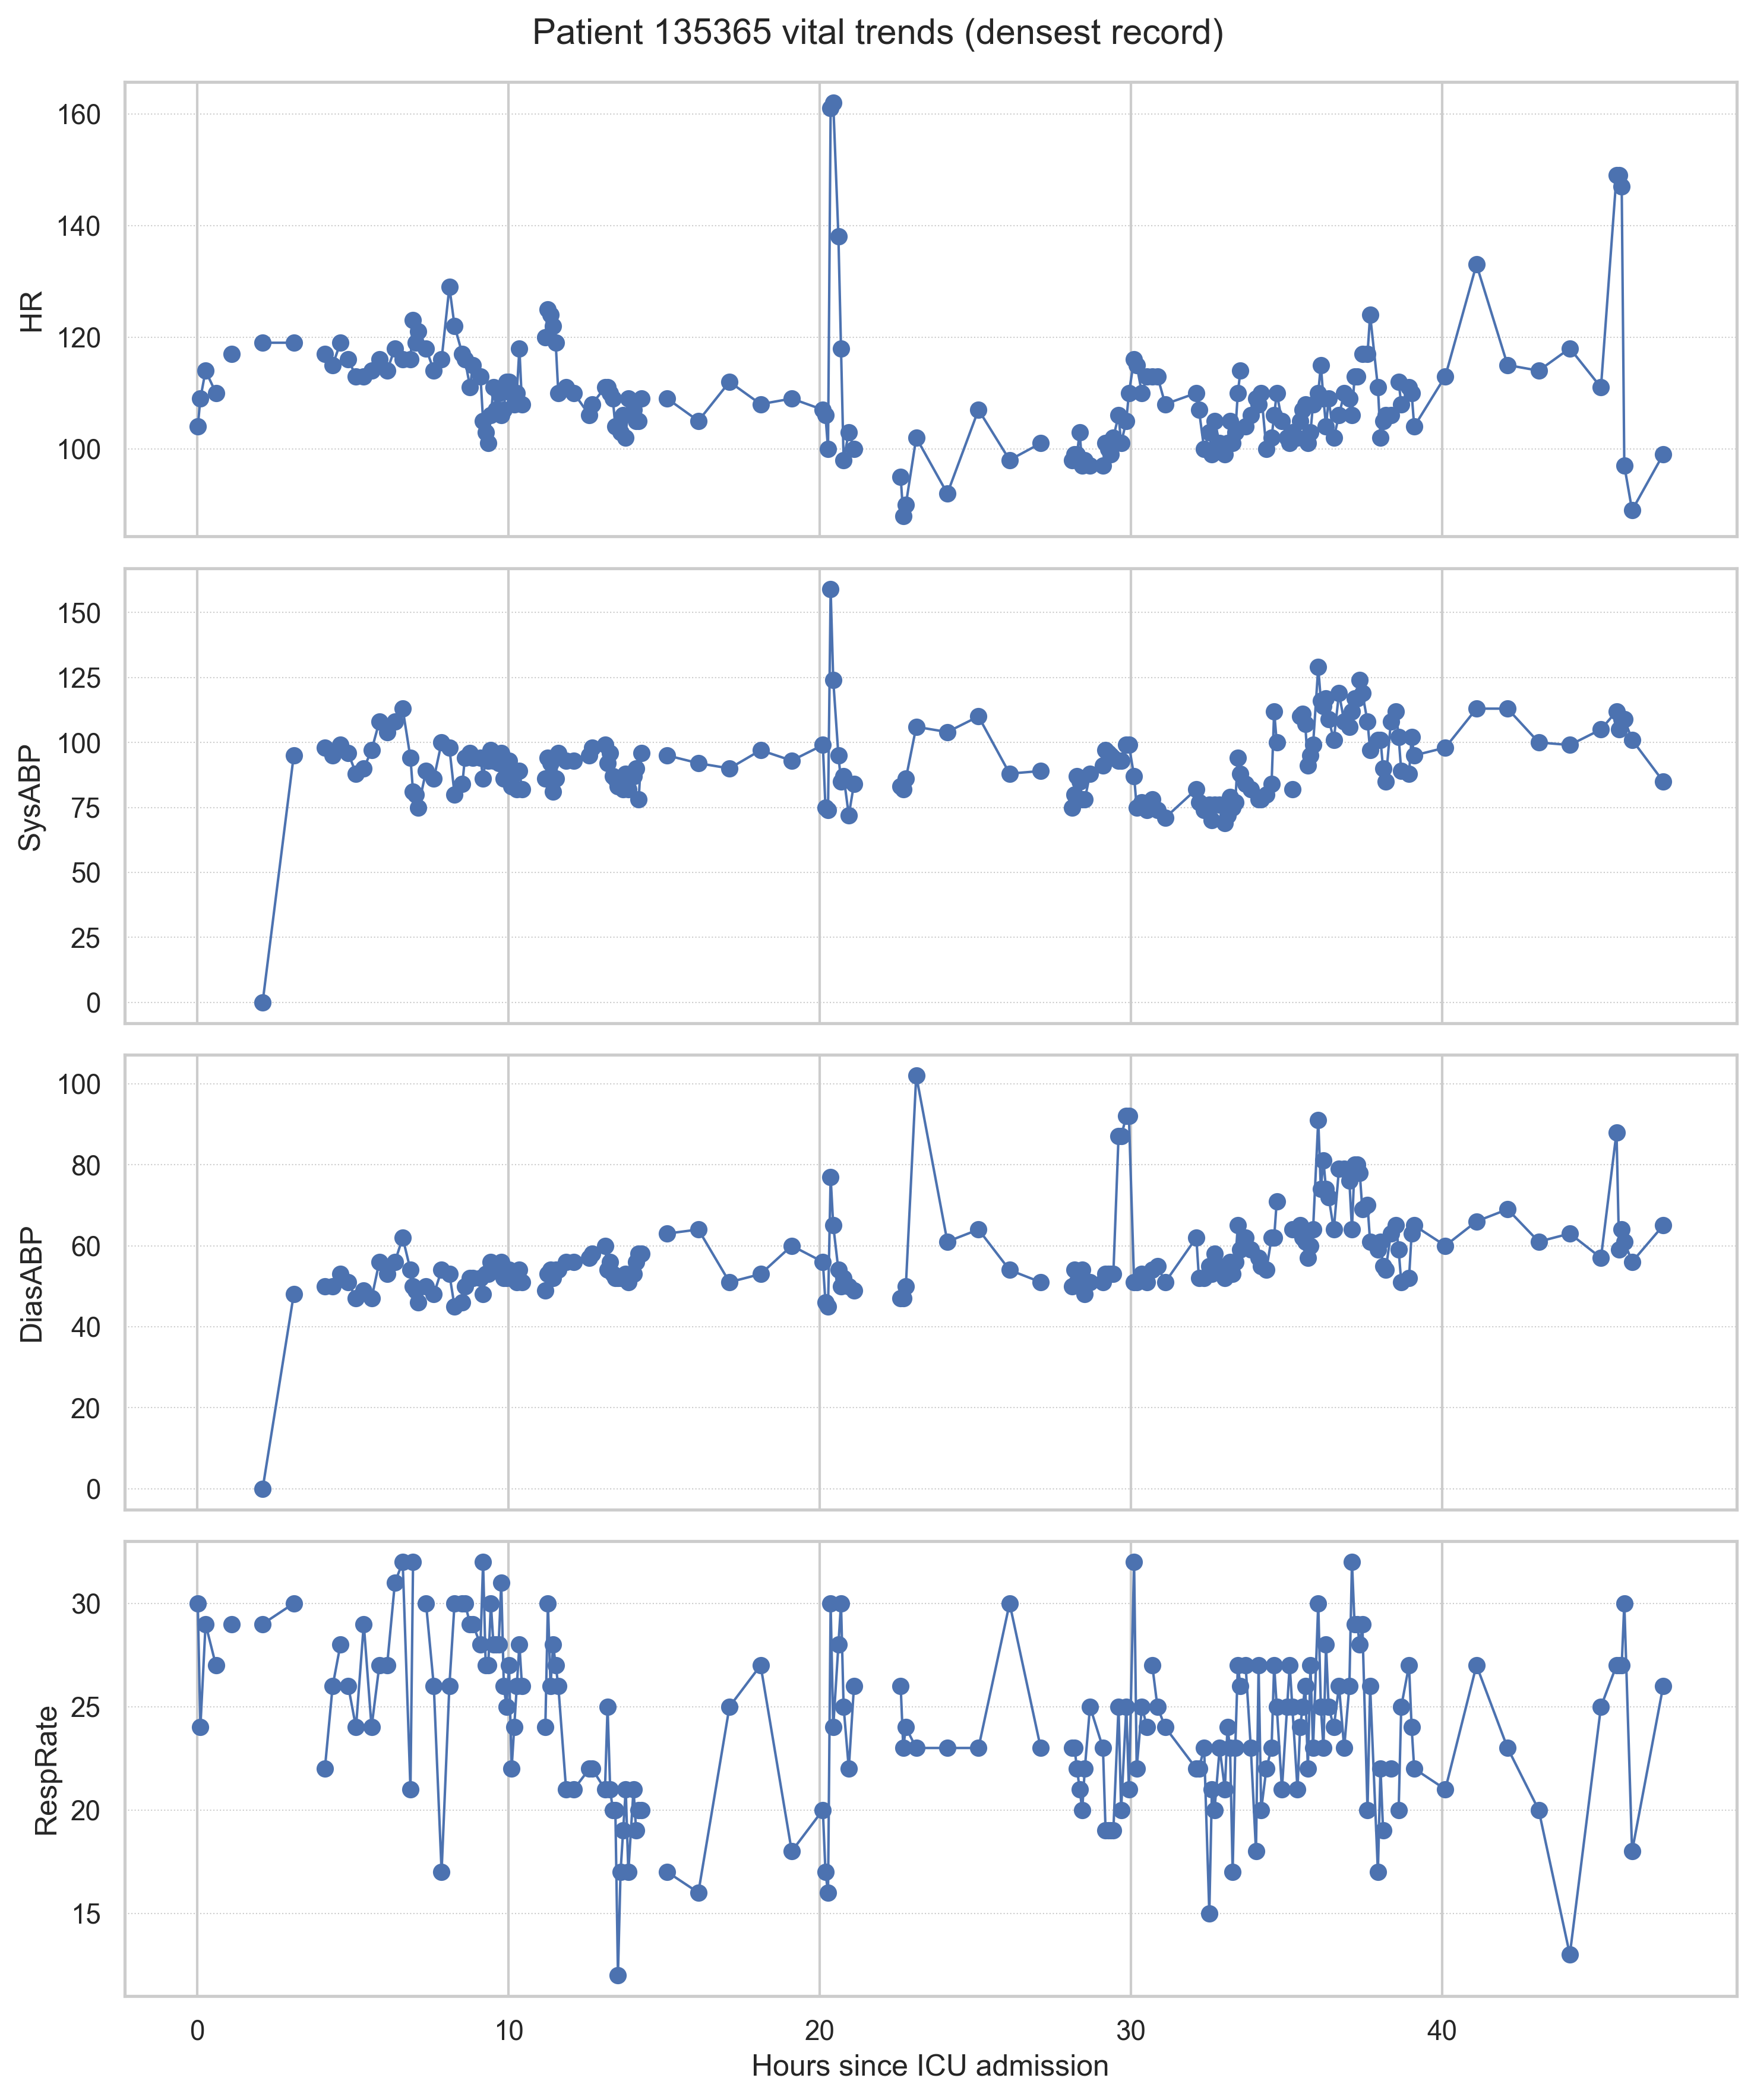
\includegraphics[width=0.9\textwidth]{figures/example_patient_vitals.png}
    \caption{Multi-panel vital sign trajectory for the densest-recorded patient.}
    \label{fig:trajectory}
\end{figure}

\section{Mortality Outcome Analysis}
\subsection{Class Balance}
Figure~\ref{fig:mortality} displays the mortality label distribution with annotated counts. The dataset remains moderately imbalanced (survivors $>$ non-survivors), guiding later modeling decisions such as class weighting.

\begin{figure}[h]
    \centering
    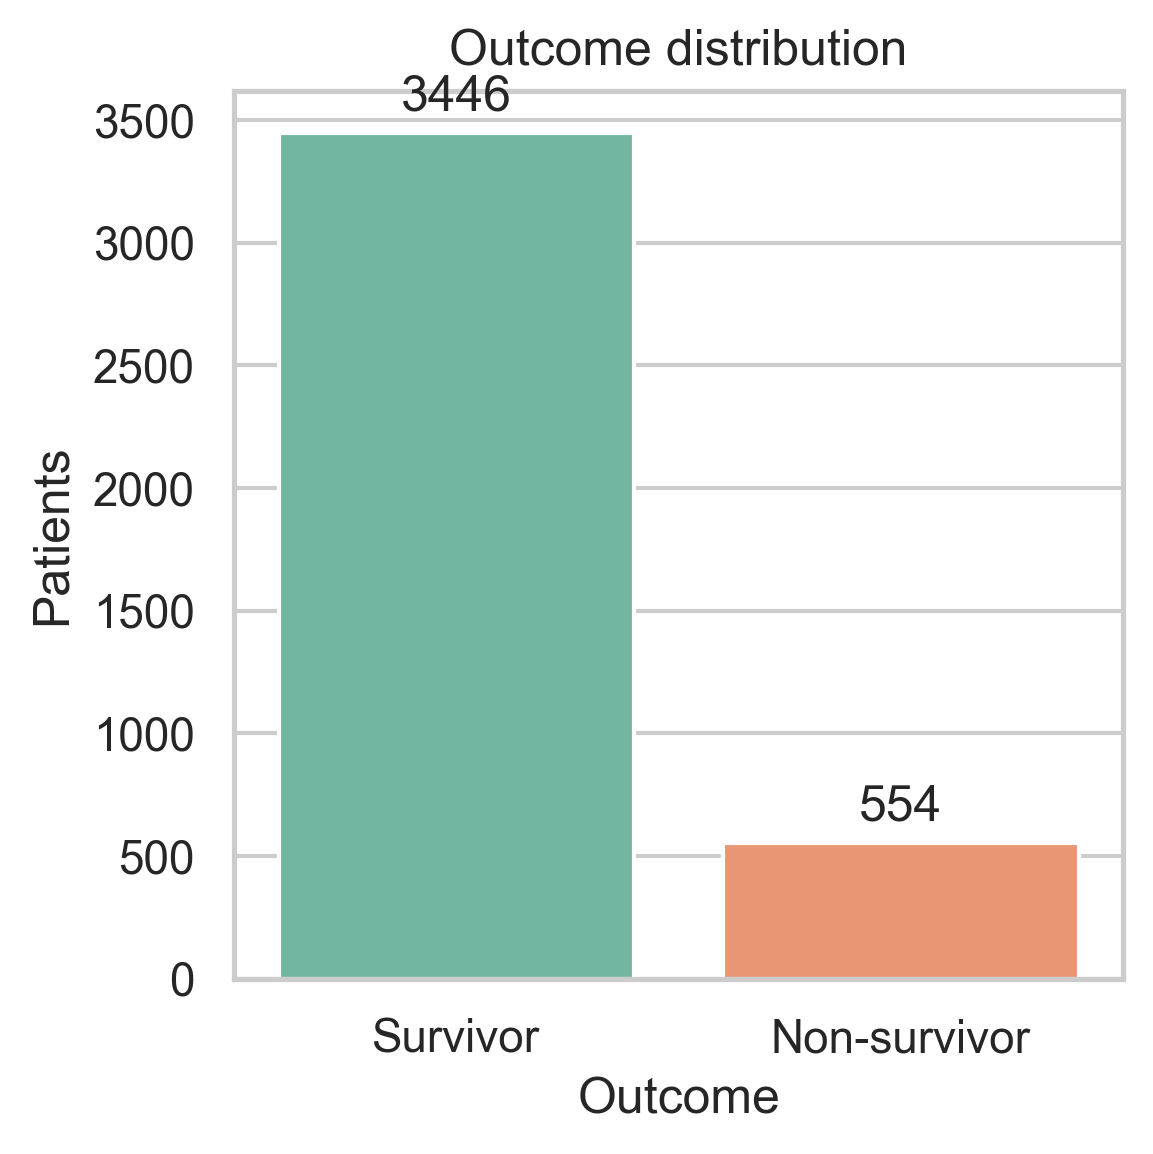
\includegraphics[width=0.55\textwidth]{figures/mortality_outcome_distribution.png}
    \caption{Outcome distribution for in-hospital mortality.}
    \label{fig:mortality}
\end{figure}

\subsection{Descriptor Shifts}
Figure~\ref{fig:kde} overlays kernel density estimates for Age, SAPS-I, and measurement counts split by outcome. Non-survivors skew older with higher SAPS-I and broader measurement coverage, suggesting both severity and monitoring intensity differ between classes.

\begin{figure}[h]
    \centering
    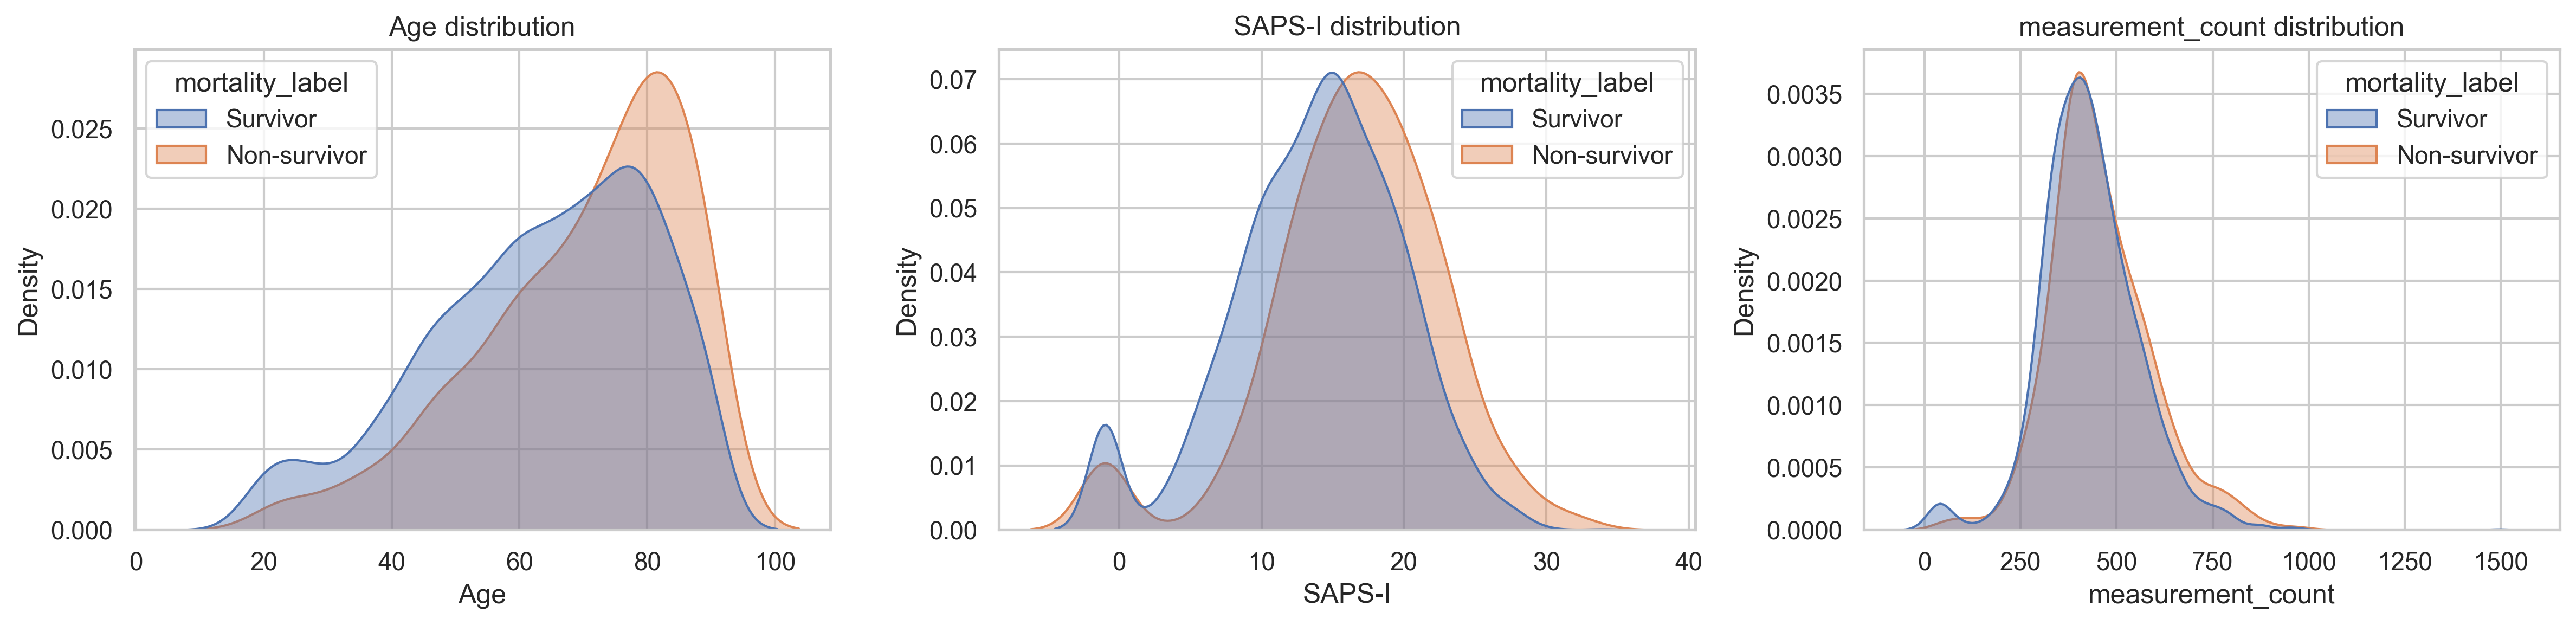
\includegraphics[width=0.9\textwidth]{figures/mortality_feature_distributions.png}
    \caption{Outcome-stratified KDEs for Age, SAPS-I, and measurement counts.}
    \label{fig:kde}
\end{figure}

\subsection{ICU-Type Interaction}
Figure~\ref{fig:icu} plots mortality within each ICU type, highlighting that medical ICUs have larger absolute counts but similar mortality rates to surgical units. This supports using ICU type as a categorical feature in predictive models.

\begin{figure}[h]
    \centering
    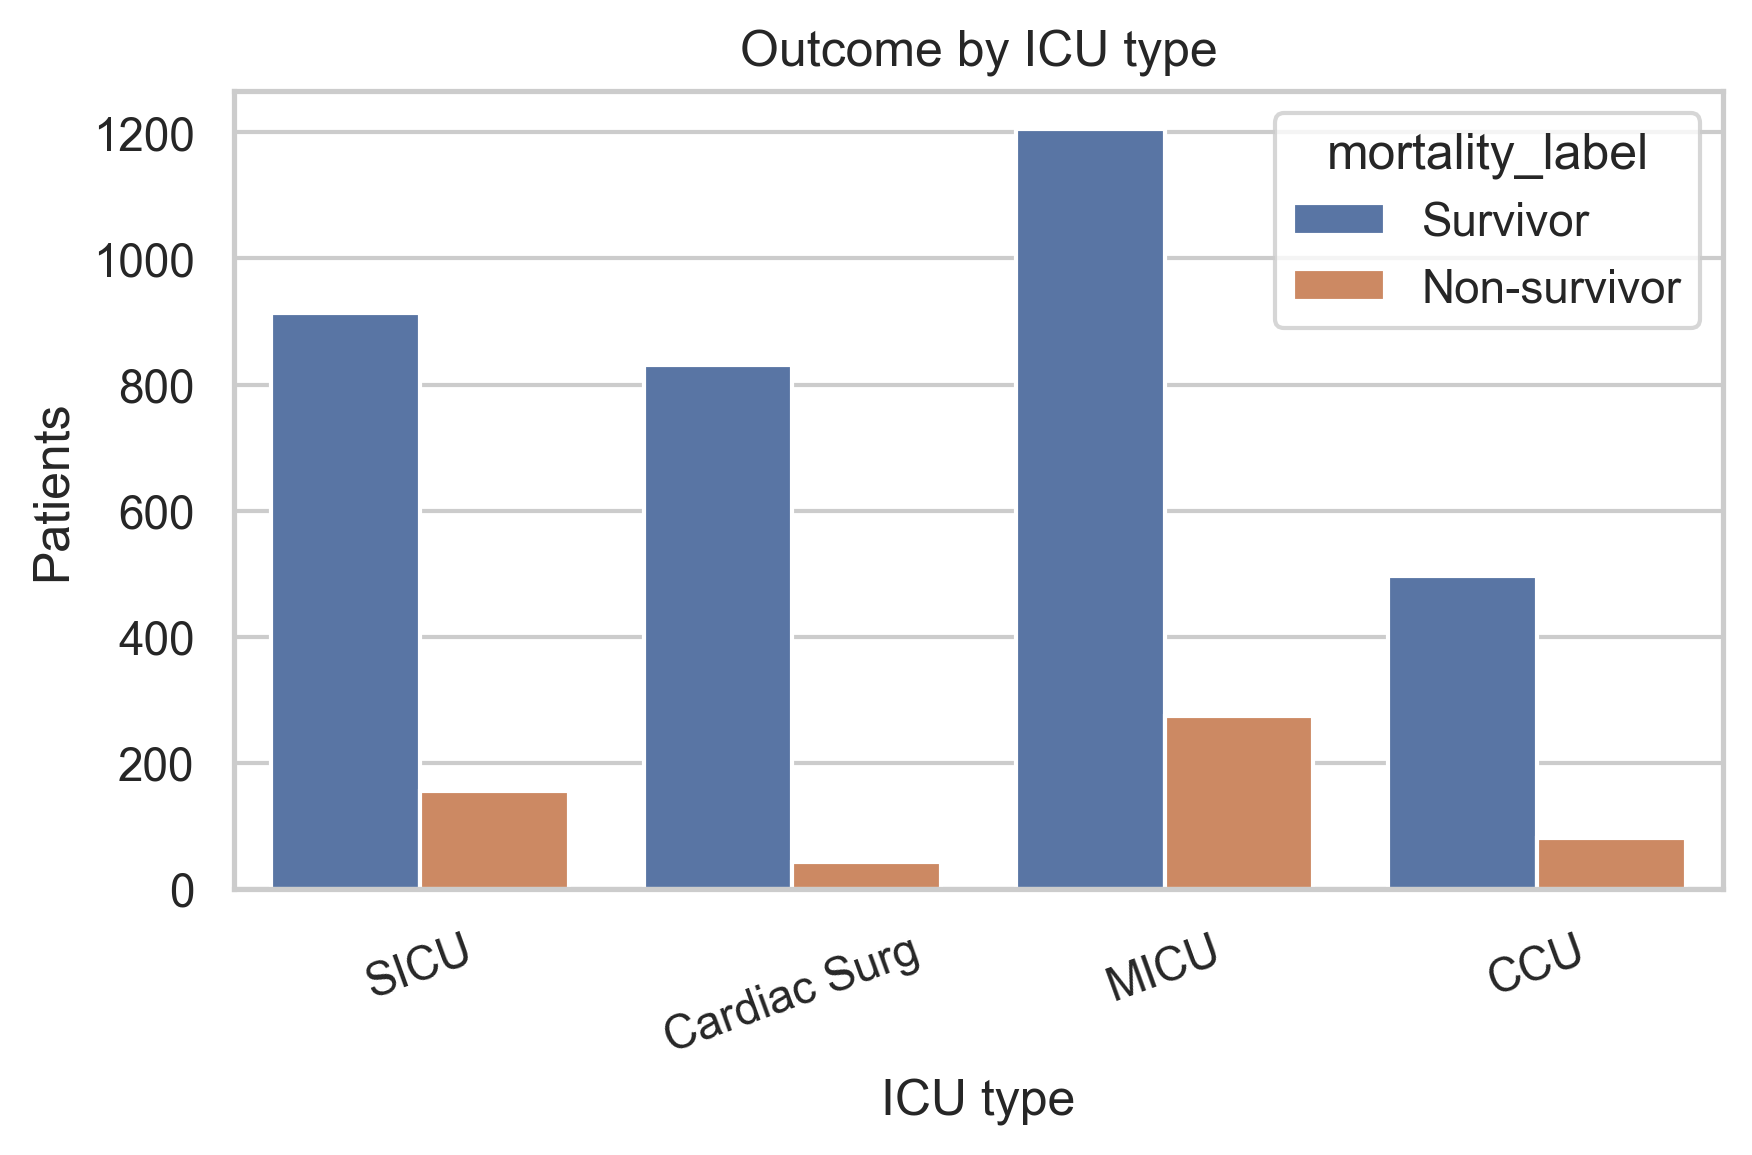
\includegraphics[width=0.65\textwidth]{figures/outcome_by_icu.png}
    \caption{Outcome breakdown conditioned on ICU type.}
    \label{fig:icu}
\end{figure}

\section{Summary Tables}
\subsection{Survival Descriptor Table}
Cell 21 of the notebook produces \texttt{survival\_summary}, a multi-index table with mean, median, and standard deviation for Age, SAPS-I, SOFA, Length of stay, and measurement counts. Presenters can export it via \texttt{survival\_summary.to\_latex()} to accompany this document. Key insights noted in the notebook:
\begin{itemize}[noitemsep]
    \item Non-survivors exhibit higher SAPS-I and SOFA scores across all summary statistics.
    \item Length of stay has a wider spread among survivors, reflecting prolonged recovery cases.
\end{itemize}

\subsection{Horizon Summary Features}
Cells 24--31 compute horizon-based aggregations (6h and 24h windows) for selected vitals/labs, impute missing entries, and log imputation metadata. Figure~\ref{fig:boxplot} visualizes four representative engineered features split by outcome, showing clear separation for MAP and SaO$_2$ metrics. The imputation plan table (\texttt{imputation\_plan\_df}) lists each feature column, category (vital/lab), missing rate, and fill value, serving as documentation for downstream model pipelines.

\begin{figure}[h]
    \centering
    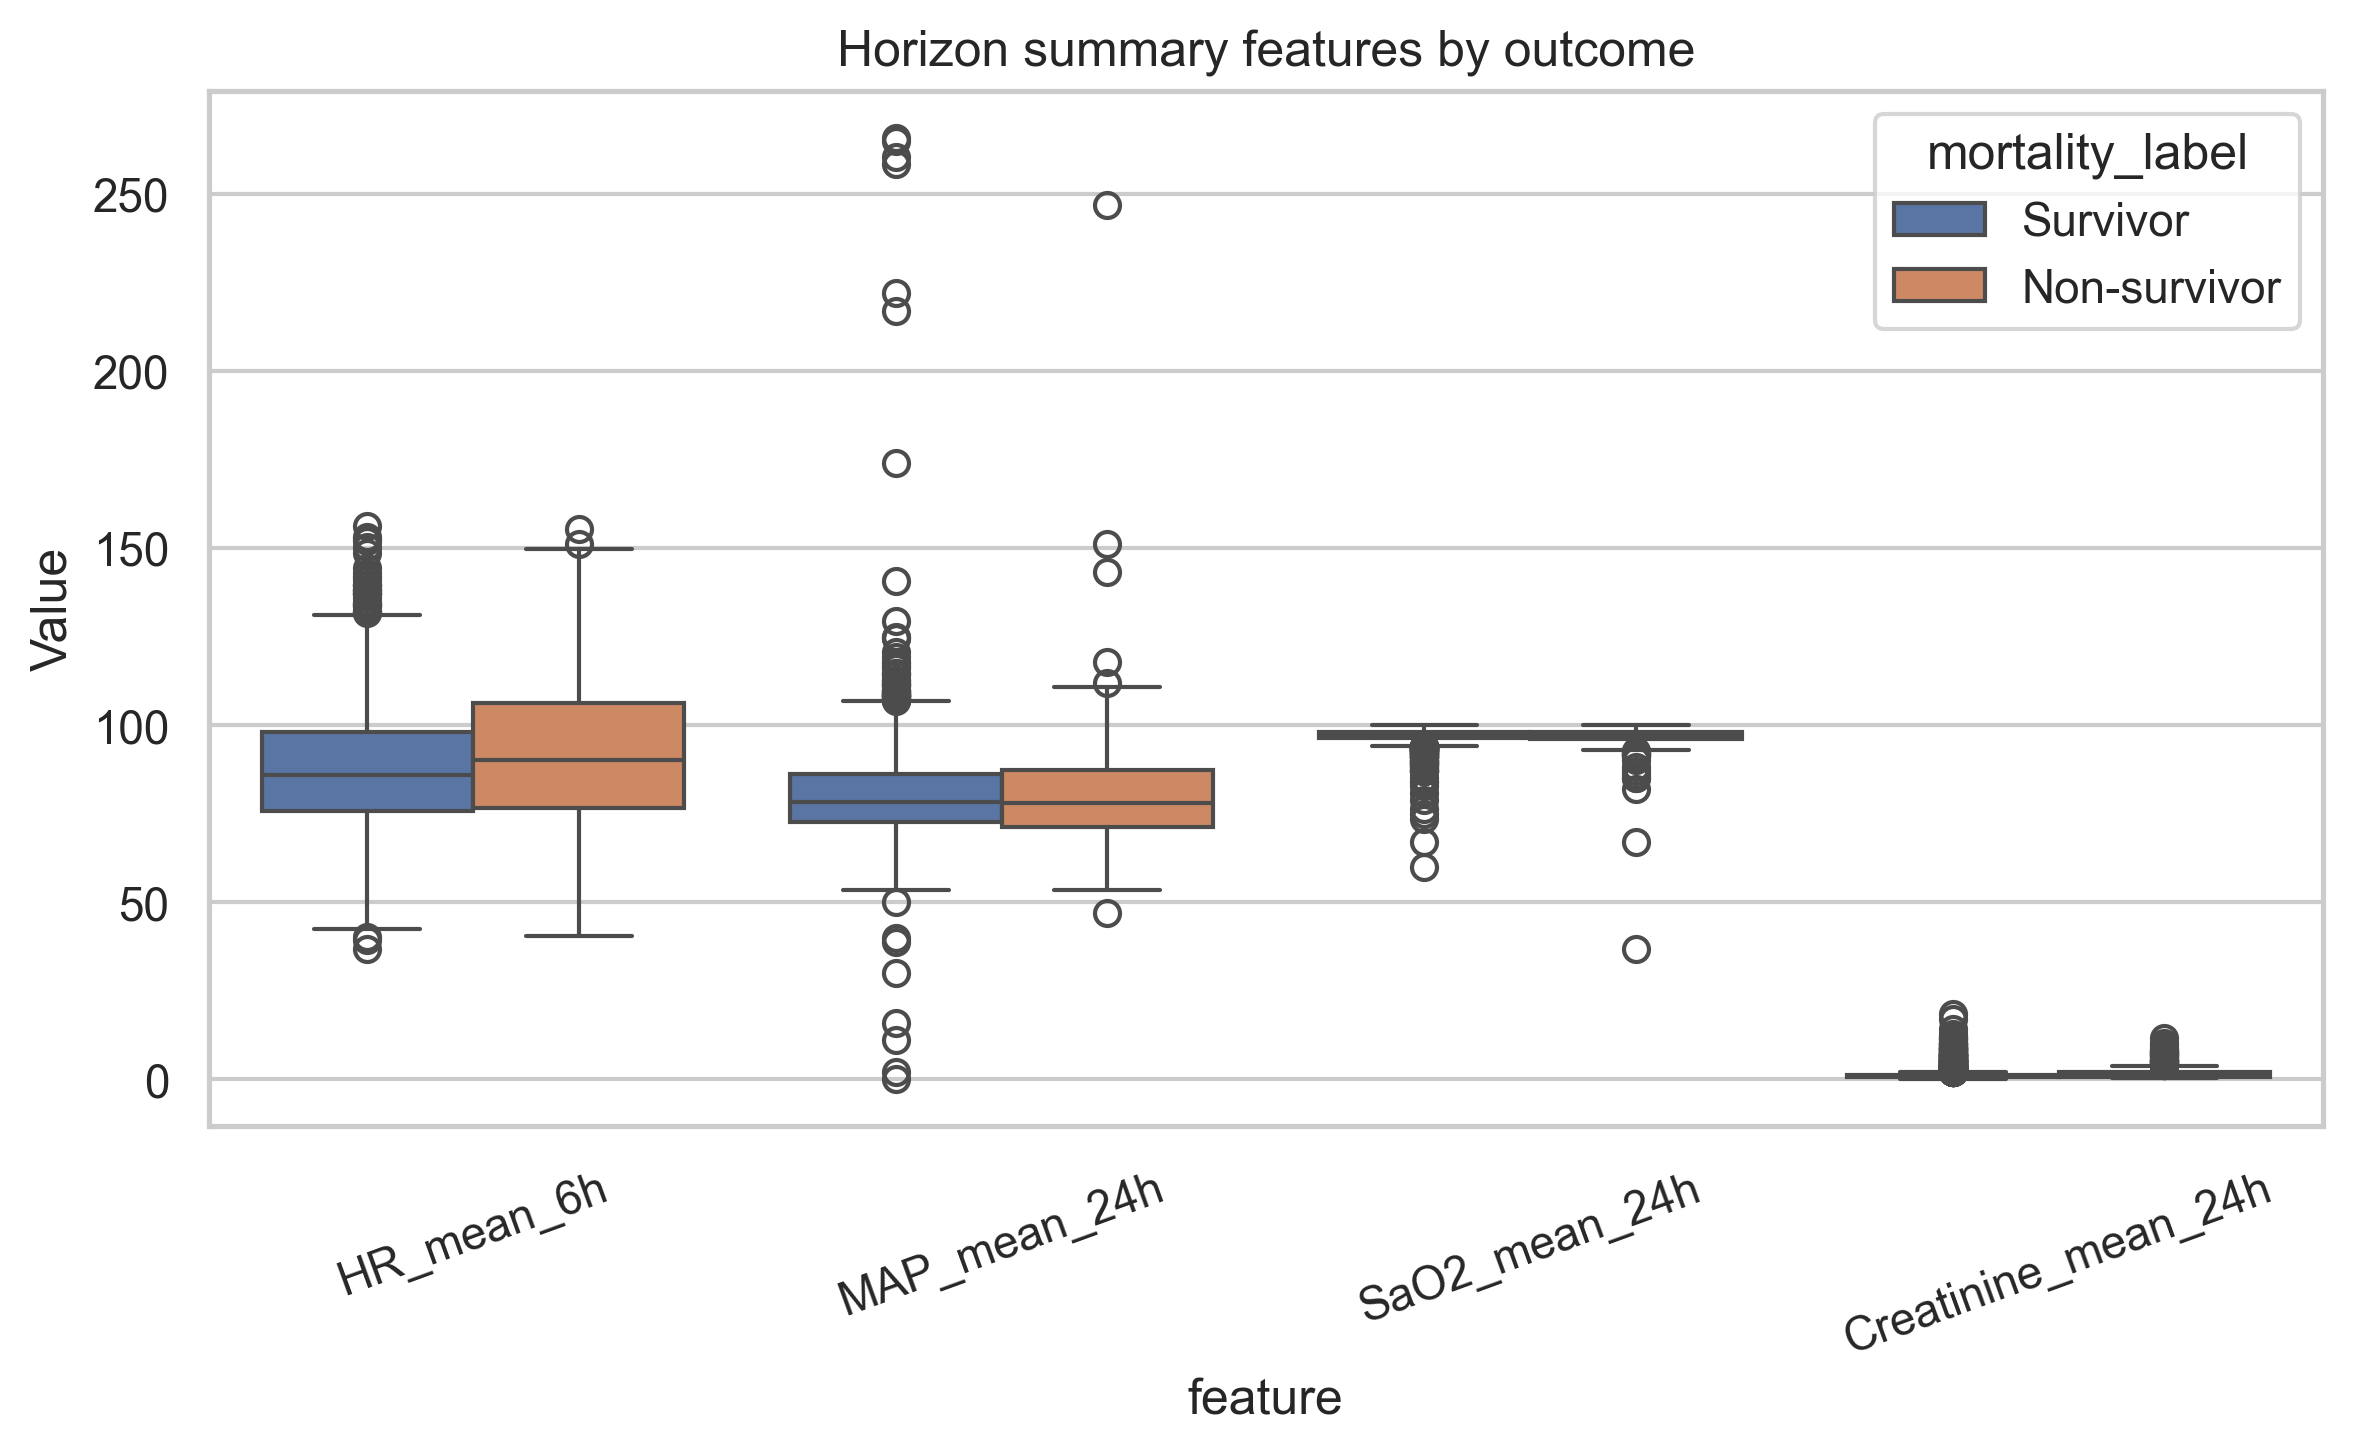
\includegraphics[width=0.8\textwidth]{figures/horizon_feature_boxplot.png}
    \caption{Boxplots of engineered 6h/24h summary features by outcome.}
    \label{fig:boxplot}
\end{figure}

\section{Reproducibility Notes}
\begin{enumerate}[noitemsep]
    \item Run \texttt{physionet\_eda.ipynb} from the project root so that relative paths resolve (data under \texttt{data/}, figures into \texttt{figures/}).
    \item All plots call \texttt{save\_figure}, which guarantees the \texttt{figures/} folder exists and logs the output path for traceability.
    \item Tables can be exported using pandas' \texttt{to\_latex()} or \texttt{to\_csv()} to integrate directly into this document if numeric values are needed.
\end{enumerate}

\section{Key Takeaways}
\begin{itemize}[noitemsep]
    \item Mortality imbalance and acuity score shifts indicate the need for calibrated classification strategies.
    \item Measurement sparsity varies drastically; modeling pipelines must incorporate masking or imputation aware of variable-level missingness rates.
    \item Horizon aggregates provide discriminative signals and should be retained in feature sets, with imputation metadata documenting any fill operations.
\end{itemize}

\end{document}
